\begin{figure}[htbp]
\section*{ POGZ}
\centering
\begin{subfigure}[b]{0.95\textwidth}
\centering
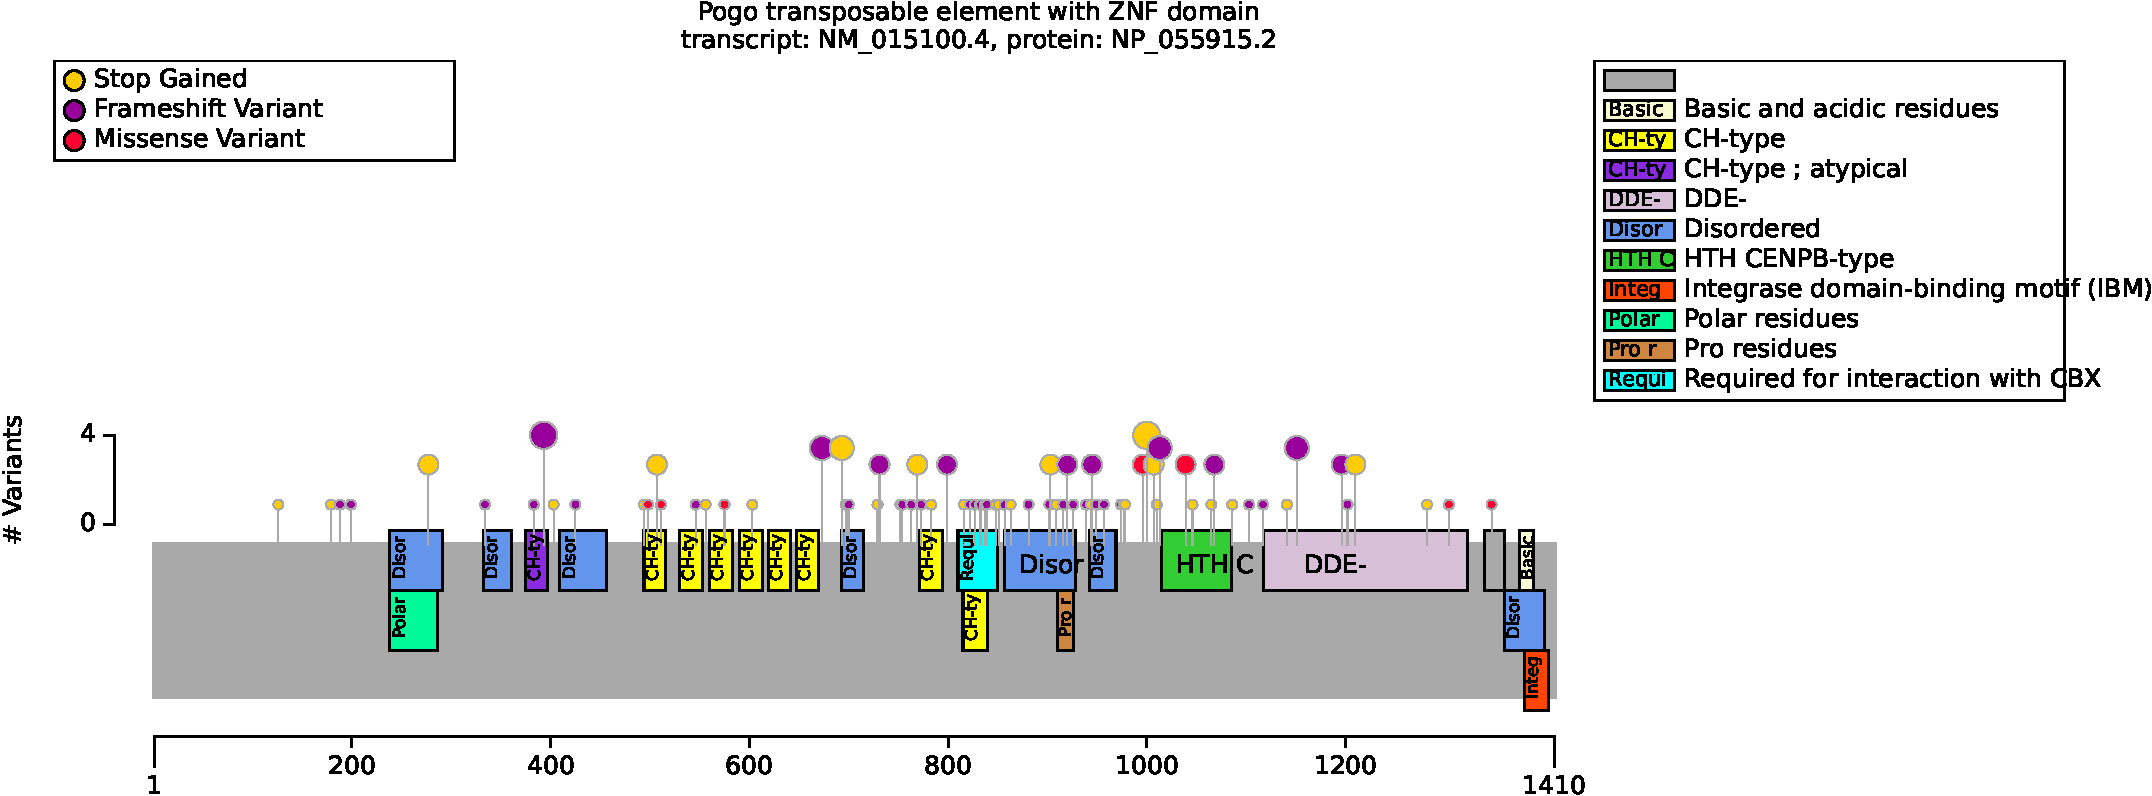
\includegraphics[width=\textwidth]{ img/POGZ_protein_diagram.pdf} 
\captionsetup{justification=raggedright,singlelinecheck=false}
\caption{Distribution of variants in POGZ}
\end{subfigure}

\vspace{2em}

\begin{subfigure}[b]{0.95\textwidth}
\centering
\resizebox{\textwidth}{!}{
\begin{tabular}{llllrr}
\toprule
Genotype (A) & Genotype (B) & total tests performed & significant results\\
\midrule
Missense & Other & 23 & 0\\
Frameshift & Other & 24 & 0\\
\bottomrule
\end{tabular}
}
\captionsetup{justification=raggedright,singlelinecheck=false}
\caption{             Fisher Exact Test performed to compare HPO annotation frequency with respect to genotypes. }
\end{subfigure}

\vspace{2em}

\begin{subfigure}[b]{0.95\textwidth}
\captionsetup{justification=raggedright,singlelinecheck=false}
\resizebox{\textwidth}{!}{
\begin{tabular}{llllrr}
\toprule
Description & Variable & Genotype (A) & Genotype (B) & p-value & xrefs\\
\midrule
A phenotypic severity score according to Nagy et al. 2022 & POGZ Severity Score & Missense & Other & 0.429 & -\\
\bottomrule
\end{tabular}
}
\caption{ POGZ Severity Score to compare Missense and Other with respect to POGZ Severity Score. }
\end{subfigure}

\vspace{2em}

\begin{subfigure}[b]{0.95\textwidth}
\captionsetup{justification=raggedright,singlelinecheck=false}
\resizebox{\textwidth}{!}{
\begin{tabular}{llllrr}
\toprule
Description & Variable & Genotype (A) & Genotype (B) & p-value & xrefs\\
\midrule
A phenotypic severity score for individuals with intellectual disability & De Vries score & Missense & Other & 0.429 & -\\
\bottomrule
\end{tabular}
}
\caption{ De Vries Score to compare Missense and Other with respect to De Vries score. }
\end{subfigure}

\vspace{2em}

\caption{ The cohort comprised 117 individuals (54 females, 62 males, 1 with unknown sex). A total of 94 HPO terms were used to annotate the cohort. Disease diagnosis: White-Sutton syndrome (OMIM:616364). Negy et al. (2022) summarized data on 117 individuals with White-Sutton syndrome. They identified a correlation 
between a severity score and nonsense-mediated RNA decay (NMD). Missense variants were more often associated with mild phenotypes 
and truncating variants predicted to escape NMD presented with more severe phenotypes. Within this group, variants in the 
proline-rich region of the POGZ protein were associated with the most severe phenotypes).
 These authors did not apply multiple testing correction \cite{PMID_35052493}.
Our analysis did not identify a significant GPC. A total of 117 unique variant alleles were found in \textit{POGZ} (transcript: \texttt{NM\_015100.4}, protein id: \texttt{NP\_055915.2}).}
\end{figure}
